\subsubsection{Numerical experiments - Estimation of $\Phi$}

\textbf{Smooth case.} We consider \eqref{eq:OneDModel} with $D = \left[ -1, 1 \right]$, the final time $T = 0.5$ and we define
\begin{align}\label{eq:FunctionsOneDSmoothPhi}
\begin{split}
	f(x) &= -V'(x), \text{ where } V(x) = 8x^4 - 8x^2 + x + 2, \\
	g(x) &= \sigma = 2.
\end{split}
\end{align}
In order to approximate $\Phi$, we perform a Montecarlo simulation using both DEM and CEM, with $M = 6 \cdot 10^5$ trajectories in order to kill the statistical error. We consider the number of timesteps for the time integration to be $N = 2^i, i = 5, \dots, 12$. Numerical results (Figure \ref{fig:KillOneDPhi}) confirm that the weak error for DEM is of order 0.5, while for CEM the order of convergence is 1.

\begin{figure}[t]
    \centering
    \begin{subfigure}{0.49\linewidth}
        \centering
        \resizebox{1\linewidth}{!}{% This file was created by matlab2tikz.
%
%The latest updates can be retrieved from
%  http://www.mathworks.com/matlabcentral/fileexchange/22022-matlab2tikz-matlab2tikz
%where you can also make suggestions and rate matlab2tikz.
%
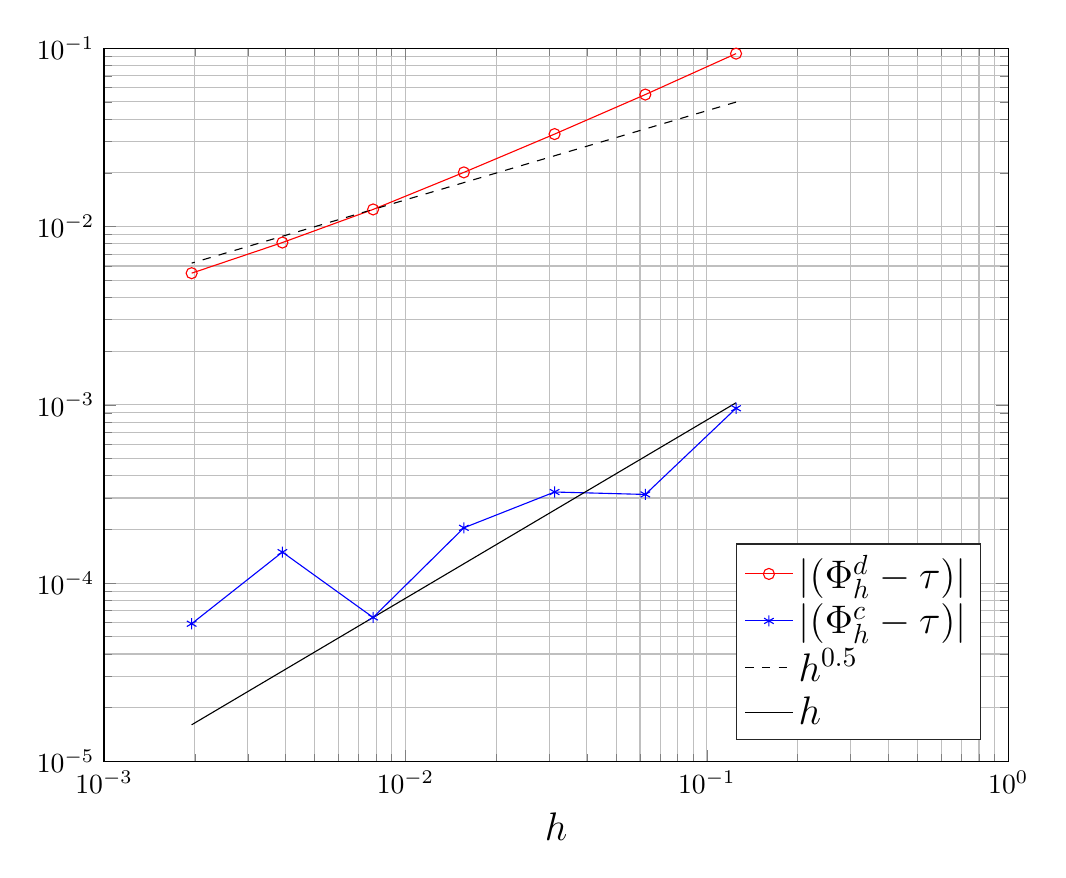
\begin{tikzpicture}

\begin{axis}[%
width=4.521in,
height=3.566in,
at={(0.758in,0.481in)},
scale only axis,
xmode=log,
xmin=0.001,
xmax=1,
xminorticks=true,
xlabel={$h$},
xlabel style={font=\Large},
xmajorgrids,
xminorgrids,
ymode=log,
ymin=1e-05,
ymax=0.1,
yminorticks=true,
ymajorgrids,
yminorgrids,
axis background/.style={fill=white},
legend pos = south east,
legend style={legend cell align=left,align=left,draw=white!15!black,font=\Large}
]
\addplot [color=red,solid,mark=o,mark options={solid}]
  table[row sep=crcr]{%
0.125	0.0931958331986392\\
0.0625	0.0549308331986392\\
0.03125	0.0329758331986393\\
0.015625	0.0201058331986392\\
0.0078125	0.0124608331986392\\
0.00390625	0.00812583319863924\\
0.001953125	0.00547083319863928\\
};
\addlegendentry{$|\E(\Phi_h^d - \tau)|$};

\addplot [color=blue,solid,mark=asterisk,mark options={solid}]
  table[row sep=crcr]{%
0.125	0.000955833198639233\\
0.0625	0.00031416680136076\\
0.03125	0.000324166801360715\\
0.015625	0.000204166801360706\\
0.0078125	6.41668013607877e-05\\
0.00390625	0.000149166801360789\\
0.001953125	5.91668013607549e-05\\
};
\addlegendentry{$|\E(\Phi_h^c - \tau)|$};

\addplot [color=black,dashed]
  table[row sep=crcr]{%
0.125	0.0498433327945569\\
0.0625	0.035244558615969\\
0.03125	0.0249216663972784\\
0.015625	0.0176222793079845\\
0.0078125	0.0124608331986392\\
0.00390625	0.00881113965399225\\
0.001953125	0.00623041659931961\\
};
\addlegendentry{$h^{0.5}$};

\addplot [color=black,solid]
  table[row sep=crcr]{%
0.125	0.0010266688217726\\
0.0625	0.000513334410886301\\
0.03125	0.000256667205443151\\
0.015625	0.000128333602721575\\
0.0078125	6.41668013607877e-05\\
0.00390625	3.20834006803938e-05\\
0.001953125	1.60417003401969e-05\\
};
\addlegendentry{$h$};

\end{axis}
\end{tikzpicture}%
 }  
        \caption{Killing boundary in $x = 1$}
        \label{fig:KillOneDPhi}
    \end{subfigure}
    \begin{subfigure}{0.49\linewidth}
        \centering
        \resizebox{1\linewidth}{!}{% This file was created by matlab2tikz.
%
%The latest updates can be retrieved from
%  http://www.mathworks.com/matlabcentral/fileexchange/22022-matlab2tikz-matlab2tikz
%where you can also make suggestions and rate matlab2tikz.
%
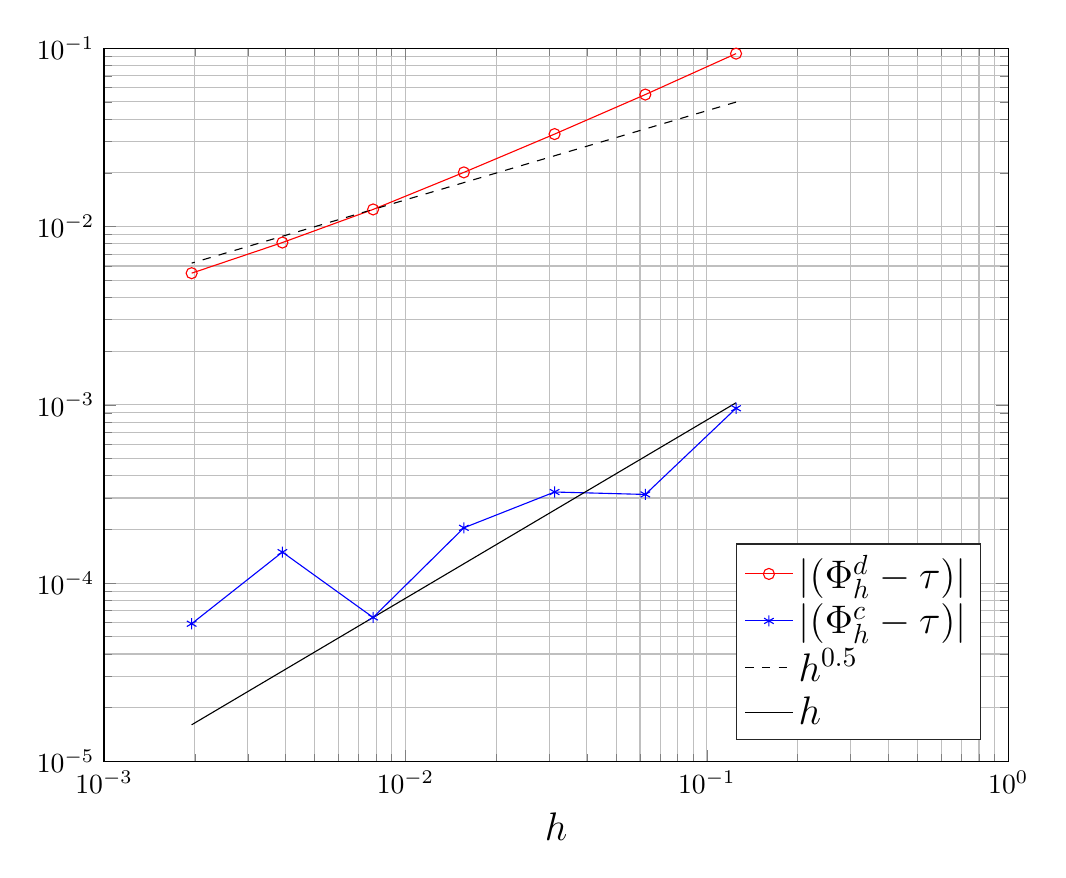
\begin{tikzpicture}

\begin{axis}[%
width=4.521in,
height=3.566in,
at={(0.758in,0.481in)},
scale only axis,
xmode=log,
xmin=0.001,
xmax=1,
xminorticks=true,
xlabel={$h$},
xlabel style={font=\Large},
xmajorgrids,
xminorgrids,
ymode=log,
ymin=1e-05,
ymax=0.1,
yminorticks=true,
ymajorgrids,
yminorgrids,
axis background/.style={fill=white},
legend pos = south east,
legend style={legend cell align=left,align=left,draw=white!15!black,font=\Large}
]
\addplot [color=red,solid,mark=o,mark options={solid}]
  table[row sep=crcr]{%
0.125	0.0931958331986392\\
0.0625	0.0549308331986392\\
0.03125	0.0329758331986393\\
0.015625	0.0201058331986392\\
0.0078125	0.0124608331986392\\
0.00390625	0.00812583319863924\\
0.001953125	0.00547083319863928\\
};
\addlegendentry{$|\E(\Phi_h^d - \tau)|$};

\addplot [color=blue,solid,mark=asterisk,mark options={solid}]
  table[row sep=crcr]{%
0.125	0.000955833198639233\\
0.0625	0.00031416680136076\\
0.03125	0.000324166801360715\\
0.015625	0.000204166801360706\\
0.0078125	6.41668013607877e-05\\
0.00390625	0.000149166801360789\\
0.001953125	5.91668013607549e-05\\
};
\addlegendentry{$|\E(\Phi_h^c - \tau)|$};

\addplot [color=black,dashed]
  table[row sep=crcr]{%
0.125	0.0498433327945569\\
0.0625	0.035244558615969\\
0.03125	0.0249216663972784\\
0.015625	0.0176222793079845\\
0.0078125	0.0124608331986392\\
0.00390625	0.00881113965399225\\
0.001953125	0.00623041659931961\\
};
\addlegendentry{$h^{0.5}$};

\addplot [color=black,solid]
  table[row sep=crcr]{%
0.125	0.0010266688217726\\
0.0625	0.000513334410886301\\
0.03125	0.000256667205443151\\
0.015625	0.000128333602721575\\
0.0078125	6.41668013607877e-05\\
0.00390625	3.20834006803938e-05\\
0.001953125	1.60417003401969e-05\\
};
\addlegendentry{$h$};

\end{axis}
\end{tikzpicture}%
 }  
        \caption{Reflecting boundary in $x = 1$}
        \label{fig:ReflectOneDPhi}
    \end{subfigure}    
    \caption{Approximation of $\Phi$. Orders of convergence of DEM and CEM in the one-dimensional case.}
    \label{fig:OrdersOneDPhi}
\end{figure}


